% Options for packages loaded elsewhere
\PassOptionsToPackage{unicode}{hyperref}
\PassOptionsToPackage{hyphens}{url}
\PassOptionsToPackage{dvipsnames,svgnames,x11names}{xcolor}
%
\documentclass[
  letterpaper,
  DIV=11,
  numbers=noendperiod]{scrartcl}

\usepackage{amsmath,amssymb}
\usepackage{iftex}
\ifPDFTeX
  \usepackage[T1]{fontenc}
  \usepackage[utf8]{inputenc}
  \usepackage{textcomp} % provide euro and other symbols
\else % if luatex or xetex
  \usepackage{unicode-math}
  \defaultfontfeatures{Scale=MatchLowercase}
  \defaultfontfeatures[\rmfamily]{Ligatures=TeX,Scale=1}
\fi
\usepackage{lmodern}
\ifPDFTeX\else  
    % xetex/luatex font selection
\fi
% Use upquote if available, for straight quotes in verbatim environments
\IfFileExists{upquote.sty}{\usepackage{upquote}}{}
\IfFileExists{microtype.sty}{% use microtype if available
  \usepackage[]{microtype}
  \UseMicrotypeSet[protrusion]{basicmath} % disable protrusion for tt fonts
}{}
\makeatletter
\@ifundefined{KOMAClassName}{% if non-KOMA class
  \IfFileExists{parskip.sty}{%
    \usepackage{parskip}
  }{% else
    \setlength{\parindent}{0pt}
    \setlength{\parskip}{6pt plus 2pt minus 1pt}}
}{% if KOMA class
  \KOMAoptions{parskip=half}}
\makeatother
\usepackage{xcolor}
\setlength{\emergencystretch}{3em} % prevent overfull lines
\setcounter{secnumdepth}{-\maxdimen} % remove section numbering
% Make \paragraph and \subparagraph free-standing
\ifx\paragraph\undefined\else
  \let\oldparagraph\paragraph
  \renewcommand{\paragraph}[1]{\oldparagraph{#1}\mbox{}}
\fi
\ifx\subparagraph\undefined\else
  \let\oldsubparagraph\subparagraph
  \renewcommand{\subparagraph}[1]{\oldsubparagraph{#1}\mbox{}}
\fi

\usepackage{color}
\usepackage{fancyvrb}
\newcommand{\VerbBar}{|}
\newcommand{\VERB}{\Verb[commandchars=\\\{\}]}
\DefineVerbatimEnvironment{Highlighting}{Verbatim}{commandchars=\\\{\}}
% Add ',fontsize=\small' for more characters per line
\usepackage{framed}
\definecolor{shadecolor}{RGB}{241,243,245}
\newenvironment{Shaded}{\begin{snugshade}}{\end{snugshade}}
\newcommand{\AlertTok}[1]{\textcolor[rgb]{0.68,0.00,0.00}{#1}}
\newcommand{\AnnotationTok}[1]{\textcolor[rgb]{0.37,0.37,0.37}{#1}}
\newcommand{\AttributeTok}[1]{\textcolor[rgb]{0.40,0.45,0.13}{#1}}
\newcommand{\BaseNTok}[1]{\textcolor[rgb]{0.68,0.00,0.00}{#1}}
\newcommand{\BuiltInTok}[1]{\textcolor[rgb]{0.00,0.23,0.31}{#1}}
\newcommand{\CharTok}[1]{\textcolor[rgb]{0.13,0.47,0.30}{#1}}
\newcommand{\CommentTok}[1]{\textcolor[rgb]{0.37,0.37,0.37}{#1}}
\newcommand{\CommentVarTok}[1]{\textcolor[rgb]{0.37,0.37,0.37}{\textit{#1}}}
\newcommand{\ConstantTok}[1]{\textcolor[rgb]{0.56,0.35,0.01}{#1}}
\newcommand{\ControlFlowTok}[1]{\textcolor[rgb]{0.00,0.23,0.31}{#1}}
\newcommand{\DataTypeTok}[1]{\textcolor[rgb]{0.68,0.00,0.00}{#1}}
\newcommand{\DecValTok}[1]{\textcolor[rgb]{0.68,0.00,0.00}{#1}}
\newcommand{\DocumentationTok}[1]{\textcolor[rgb]{0.37,0.37,0.37}{\textit{#1}}}
\newcommand{\ErrorTok}[1]{\textcolor[rgb]{0.68,0.00,0.00}{#1}}
\newcommand{\ExtensionTok}[1]{\textcolor[rgb]{0.00,0.23,0.31}{#1}}
\newcommand{\FloatTok}[1]{\textcolor[rgb]{0.68,0.00,0.00}{#1}}
\newcommand{\FunctionTok}[1]{\textcolor[rgb]{0.28,0.35,0.67}{#1}}
\newcommand{\ImportTok}[1]{\textcolor[rgb]{0.00,0.46,0.62}{#1}}
\newcommand{\InformationTok}[1]{\textcolor[rgb]{0.37,0.37,0.37}{#1}}
\newcommand{\KeywordTok}[1]{\textcolor[rgb]{0.00,0.23,0.31}{#1}}
\newcommand{\NormalTok}[1]{\textcolor[rgb]{0.00,0.23,0.31}{#1}}
\newcommand{\OperatorTok}[1]{\textcolor[rgb]{0.37,0.37,0.37}{#1}}
\newcommand{\OtherTok}[1]{\textcolor[rgb]{0.00,0.23,0.31}{#1}}
\newcommand{\PreprocessorTok}[1]{\textcolor[rgb]{0.68,0.00,0.00}{#1}}
\newcommand{\RegionMarkerTok}[1]{\textcolor[rgb]{0.00,0.23,0.31}{#1}}
\newcommand{\SpecialCharTok}[1]{\textcolor[rgb]{0.37,0.37,0.37}{#1}}
\newcommand{\SpecialStringTok}[1]{\textcolor[rgb]{0.13,0.47,0.30}{#1}}
\newcommand{\StringTok}[1]{\textcolor[rgb]{0.13,0.47,0.30}{#1}}
\newcommand{\VariableTok}[1]{\textcolor[rgb]{0.07,0.07,0.07}{#1}}
\newcommand{\VerbatimStringTok}[1]{\textcolor[rgb]{0.13,0.47,0.30}{#1}}
\newcommand{\WarningTok}[1]{\textcolor[rgb]{0.37,0.37,0.37}{\textit{#1}}}

\providecommand{\tightlist}{%
  \setlength{\itemsep}{0pt}\setlength{\parskip}{0pt}}\usepackage{longtable,booktabs,array}
\usepackage{calc} % for calculating minipage widths
% Correct order of tables after \paragraph or \subparagraph
\usepackage{etoolbox}
\makeatletter
\patchcmd\longtable{\par}{\if@noskipsec\mbox{}\fi\par}{}{}
\makeatother
% Allow footnotes in longtable head/foot
\IfFileExists{footnotehyper.sty}{\usepackage{footnotehyper}}{\usepackage{footnote}}
\makesavenoteenv{longtable}
\usepackage{graphicx}
\makeatletter
\def\maxwidth{\ifdim\Gin@nat@width>\linewidth\linewidth\else\Gin@nat@width\fi}
\def\maxheight{\ifdim\Gin@nat@height>\textheight\textheight\else\Gin@nat@height\fi}
\makeatother
% Scale images if necessary, so that they will not overflow the page
% margins by default, and it is still possible to overwrite the defaults
% using explicit options in \includegraphics[width, height, ...]{}
\setkeys{Gin}{width=\maxwidth,height=\maxheight,keepaspectratio}
% Set default figure placement to htbp
\makeatletter
\def\fps@figure{htbp}
\makeatother

\KOMAoption{captions}{tableheading}
\makeatletter
\makeatother
\makeatletter
\makeatother
\makeatletter
\@ifpackageloaded{caption}{}{\usepackage{caption}}
\AtBeginDocument{%
\ifdefined\contentsname
  \renewcommand*\contentsname{Table of contents}
\else
  \newcommand\contentsname{Table of contents}
\fi
\ifdefined\listfigurename
  \renewcommand*\listfigurename{List of Figures}
\else
  \newcommand\listfigurename{List of Figures}
\fi
\ifdefined\listtablename
  \renewcommand*\listtablename{List of Tables}
\else
  \newcommand\listtablename{List of Tables}
\fi
\ifdefined\figurename
  \renewcommand*\figurename{Figure}
\else
  \newcommand\figurename{Figure}
\fi
\ifdefined\tablename
  \renewcommand*\tablename{Table}
\else
  \newcommand\tablename{Table}
\fi
}
\@ifpackageloaded{float}{}{\usepackage{float}}
\floatstyle{ruled}
\@ifundefined{c@chapter}{\newfloat{codelisting}{h}{lop}}{\newfloat{codelisting}{h}{lop}[chapter]}
\floatname{codelisting}{Listing}
\newcommand*\listoflistings{\listof{codelisting}{List of Listings}}
\makeatother
\makeatletter
\@ifpackageloaded{caption}{}{\usepackage{caption}}
\@ifpackageloaded{subcaption}{}{\usepackage{subcaption}}
\makeatother
\makeatletter
\@ifpackageloaded{tcolorbox}{}{\usepackage[skins,breakable]{tcolorbox}}
\makeatother
\makeatletter
\@ifundefined{shadecolor}{\definecolor{shadecolor}{rgb}{.97, .97, .97}}
\makeatother
\makeatletter
\makeatother
\makeatletter
\makeatother
\ifLuaTeX
  \usepackage{selnolig}  % disable illegal ligatures
\fi
\IfFileExists{bookmark.sty}{\usepackage{bookmark}}{\usepackage{hyperref}}
\IfFileExists{xurl.sty}{\usepackage{xurl}}{} % add URL line breaks if available
\urlstyle{same} % disable monospaced font for URLs
\hypersetup{
  pdftitle={Class 9: Halloween Mini-Project},
  pdfauthor={Raquel Gonzalez (A16207442)},
  colorlinks=true,
  linkcolor={blue},
  filecolor={Maroon},
  citecolor={Blue},
  urlcolor={Blue},
  pdfcreator={LaTeX via pandoc}}

\title{Class 9: Halloween Mini-Project}
\author{Raquel Gonzalez (A16207442)}
\date{}

\begin{document}
\maketitle
\ifdefined\Shaded\renewenvironment{Shaded}{\begin{tcolorbox}[interior hidden, breakable, frame hidden, borderline west={3pt}{0pt}{shadecolor}, enhanced, boxrule=0pt, sharp corners]}{\end{tcolorbox}}\fi

Here we analyze a candy dataset from the 538 website. This is a CSV file
from their GitHub repository.

\hypertarget{data-import}{%
\subsection{Data Import}\label{data-import}}

\begin{Shaded}
\begin{Highlighting}[]
\NormalTok{candy }\OtherTok{\textless{}{-}} \FunctionTok{read.csv}\NormalTok{(}\StringTok{"candy{-}data.csv"}\NormalTok{, }\AttributeTok{row.names =} \DecValTok{1}\NormalTok{)}
\FunctionTok{head}\NormalTok{(candy)}
\end{Highlighting}
\end{Shaded}

\begin{verbatim}
             chocolate fruity caramel peanutyalmondy nougat crispedricewafer
100 Grand            1      0       1              0      0                1
3 Musketeers         1      0       0              0      1                0
One dime             0      0       0              0      0                0
One quarter          0      0       0              0      0                0
Air Heads            0      1       0              0      0                0
Almond Joy           1      0       0              1      0                0
             hard bar pluribus sugarpercent pricepercent winpercent
100 Grand       0   1        0        0.732        0.860   66.97173
3 Musketeers    0   1        0        0.604        0.511   67.60294
One dime        0   0        0        0.011        0.116   32.26109
One quarter     0   0        0        0.011        0.511   46.11650
Air Heads       0   0        0        0.906        0.511   52.34146
Almond Joy      0   1        0        0.465        0.767   50.34755
\end{verbatim}

\begin{quote}
Q1: How many different candy types are in this dataset?
\end{quote}

\begin{Shaded}
\begin{Highlighting}[]
\FunctionTok{nrow}\NormalTok{(candy)}
\end{Highlighting}
\end{Shaded}

\begin{verbatim}
[1] 85
\end{verbatim}

There are 85 different candy types in this dataset

\begin{quote}
Q2: How many fruity candy types are in the dataset?
\end{quote}

\begin{Shaded}
\begin{Highlighting}[]
\FunctionTok{sum}\NormalTok{(candy}\SpecialCharTok{$}\NormalTok{fruity)}
\end{Highlighting}
\end{Shaded}

\begin{verbatim}
[1] 38
\end{verbatim}

There are 38 fruity candy types in the dataset.

\hypertarget{data-exploration}{%
\subsection{Data Exploration}\label{data-exploration}}

\begin{quote}
Q3: What is your favorite candy in the dataset and what is its
\texttt{winpercent} value?
\end{quote}

\begin{Shaded}
\begin{Highlighting}[]
\NormalTok{candy[}\StringTok{"Sour Patch Kids"}\NormalTok{,]}\SpecialCharTok{$}\NormalTok{winpercent}
\end{Highlighting}
\end{Shaded}

\begin{verbatim}
[1] 59.864
\end{verbatim}

My favorite candy is Sour Patch Kids. Its win percent is 59.86\%.

\begin{quote}
Q4: What is the \texttt{winpercent} value for ``Kit Kat''
\end{quote}

\begin{Shaded}
\begin{Highlighting}[]
\NormalTok{candy[}\StringTok{"Kit Kat"}\NormalTok{,]}\SpecialCharTok{$}\NormalTok{winpercent}
\end{Highlighting}
\end{Shaded}

\begin{verbatim}
[1] 76.7686
\end{verbatim}

The win percent for Kit Kat is 76.77\%

\begin{quote}
Q5: What is the \texttt{winpercent} value for ``Tootsie Roll Snack
Bars''?
\end{quote}

\begin{Shaded}
\begin{Highlighting}[]
\NormalTok{candy[}\StringTok{"Tootsie Roll Snack Bars"}\NormalTok{,]}\SpecialCharTok{$}\NormalTok{winpercent}
\end{Highlighting}
\end{Shaded}

\begin{verbatim}
[1] 49.6535
\end{verbatim}

The win percent for Tootsie Roll Snack Bars is 49.65\%

\begin{quote}
Q: What is the least liked candy in the dataset - lowest winpercent?
\end{quote}

\begin{Shaded}
\begin{Highlighting}[]
\NormalTok{inds }\OtherTok{\textless{}{-}} \FunctionTok{order}\NormalTok{(candy}\SpecialCharTok{$}\NormalTok{winpercent)}
\FunctionTok{head}\NormalTok{(candy[inds,])}
\end{Highlighting}
\end{Shaded}

\begin{verbatim}
                   chocolate fruity caramel peanutyalmondy nougat
Nik L Nip                  0      1       0              0      0
Boston Baked Beans         0      0       0              1      0
Chiclets                   0      1       0              0      0
Super Bubble               0      1       0              0      0
Jawbusters                 0      1       0              0      0
Root Beer Barrels          0      0       0              0      0
                   crispedricewafer hard bar pluribus sugarpercent pricepercent
Nik L Nip                         0    0   0        1        0.197        0.976
Boston Baked Beans                0    0   0        1        0.313        0.511
Chiclets                          0    0   0        1        0.046        0.325
Super Bubble                      0    0   0        0        0.162        0.116
Jawbusters                        0    1   0        1        0.093        0.511
Root Beer Barrels                 0    1   0        1        0.732        0.069
                   winpercent
Nik L Nip            22.44534
Boston Baked Beans   23.41782
Chiclets             24.52499
Super Bubble         27.30386
Jawbusters           28.12744
Root Beer Barrels    29.70369
\end{verbatim}

The least liked candy is Nik L Nip with a win percent of 22.45\%

\begin{Shaded}
\begin{Highlighting}[]
\FunctionTok{library}\NormalTok{(skimr)}
\FunctionTok{skim}\NormalTok{(candy)}
\end{Highlighting}
\end{Shaded}

\begin{longtable}[]{@{}ll@{}}
\caption{Data summary}\tabularnewline
\toprule\noalign{}
\endfirsthead
\endhead
\bottomrule\noalign{}
\endlastfoot
Name & candy \\
Number of rows & 85 \\
Number of columns & 12 \\
\_\_\_\_\_\_\_\_\_\_\_\_\_\_\_\_\_\_\_\_\_\_\_ & \\
Column type frequency: & \\
numeric & 12 \\
\_\_\_\_\_\_\_\_\_\_\_\_\_\_\_\_\_\_\_\_\_\_\_\_ & \\
Group variables & None \\
\end{longtable}

\textbf{Variable type: numeric}

\begin{longtable}[]{@{}
  >{\raggedright\arraybackslash}p{(\columnwidth - 20\tabcolsep) * \real{0.1910}}
  >{\raggedleft\arraybackslash}p{(\columnwidth - 20\tabcolsep) * \real{0.1124}}
  >{\raggedleft\arraybackslash}p{(\columnwidth - 20\tabcolsep) * \real{0.1573}}
  >{\raggedleft\arraybackslash}p{(\columnwidth - 20\tabcolsep) * \real{0.0674}}
  >{\raggedleft\arraybackslash}p{(\columnwidth - 20\tabcolsep) * \real{0.0674}}
  >{\raggedleft\arraybackslash}p{(\columnwidth - 20\tabcolsep) * \real{0.0674}}
  >{\raggedleft\arraybackslash}p{(\columnwidth - 20\tabcolsep) * \real{0.0674}}
  >{\raggedleft\arraybackslash}p{(\columnwidth - 20\tabcolsep) * \real{0.0674}}
  >{\raggedleft\arraybackslash}p{(\columnwidth - 20\tabcolsep) * \real{0.0674}}
  >{\raggedleft\arraybackslash}p{(\columnwidth - 20\tabcolsep) * \real{0.0674}}
  >{\raggedright\arraybackslash}p{(\columnwidth - 20\tabcolsep) * \real{0.0674}}@{}}
\toprule\noalign{}
\begin{minipage}[b]{\linewidth}\raggedright
skim\_variable
\end{minipage} & \begin{minipage}[b]{\linewidth}\raggedleft
n\_missing
\end{minipage} & \begin{minipage}[b]{\linewidth}\raggedleft
complete\_rate
\end{minipage} & \begin{minipage}[b]{\linewidth}\raggedleft
mean
\end{minipage} & \begin{minipage}[b]{\linewidth}\raggedleft
sd
\end{minipage} & \begin{minipage}[b]{\linewidth}\raggedleft
p0
\end{minipage} & \begin{minipage}[b]{\linewidth}\raggedleft
p25
\end{minipage} & \begin{minipage}[b]{\linewidth}\raggedleft
p50
\end{minipage} & \begin{minipage}[b]{\linewidth}\raggedleft
p75
\end{minipage} & \begin{minipage}[b]{\linewidth}\raggedleft
p100
\end{minipage} & \begin{minipage}[b]{\linewidth}\raggedright
hist
\end{minipage} \\
\midrule\noalign{}
\endhead
\bottomrule\noalign{}
\endlastfoot
chocolate & 0 & 1 & 0.44 & 0.50 & 0.00 & 0.00 & 0.00 & 1.00 & 1.00 &
▇▁▁▁▆ \\
fruity & 0 & 1 & 0.45 & 0.50 & 0.00 & 0.00 & 0.00 & 1.00 & 1.00 &
▇▁▁▁▆ \\
caramel & 0 & 1 & 0.16 & 0.37 & 0.00 & 0.00 & 0.00 & 0.00 & 1.00 &
▇▁▁▁▂ \\
peanutyalmondy & 0 & 1 & 0.16 & 0.37 & 0.00 & 0.00 & 0.00 & 0.00 & 1.00
& ▇▁▁▁▂ \\
nougat & 0 & 1 & 0.08 & 0.28 & 0.00 & 0.00 & 0.00 & 0.00 & 1.00 &
▇▁▁▁▁ \\
crispedricewafer & 0 & 1 & 0.08 & 0.28 & 0.00 & 0.00 & 0.00 & 0.00 &
1.00 & ▇▁▁▁▁ \\
hard & 0 & 1 & 0.18 & 0.38 & 0.00 & 0.00 & 0.00 & 0.00 & 1.00 & ▇▁▁▁▂ \\
bar & 0 & 1 & 0.25 & 0.43 & 0.00 & 0.00 & 0.00 & 0.00 & 1.00 & ▇▁▁▁▂ \\
pluribus & 0 & 1 & 0.52 & 0.50 & 0.00 & 0.00 & 1.00 & 1.00 & 1.00 &
▇▁▁▁▇ \\
sugarpercent & 0 & 1 & 0.48 & 0.28 & 0.01 & 0.22 & 0.47 & 0.73 & 0.99 &
▇▇▇▇▆ \\
pricepercent & 0 & 1 & 0.47 & 0.29 & 0.01 & 0.26 & 0.47 & 0.65 & 0.98 &
▇▇▇▇▆ \\
winpercent & 0 & 1 & 50.32 & 14.71 & 22.45 & 39.14 & 47.83 & 59.86 &
84.18 & ▃▇▆▅▂ \\
\end{longtable}

\begin{quote}
Q6: Is there any variable/column that looks to be on a different scale
to the majority of the other columns in the dataset?
\end{quote}

The row \texttt{winpercent} looks to be on a different scale (much
larger) to the majority of the other columns in the dataset.

\begin{quote}
Q7: What do you think a zero and one represent for the
\texttt{candy\$chocolate} column?
\end{quote}

Zero and One represent True/False values. The candy gets a zero if it is
not chocolate (false) and a one if it is chocolate (true).

\begin{quote}
Q8: Plot a histogram of winpercent values
\end{quote}

\begin{Shaded}
\begin{Highlighting}[]
\FunctionTok{library}\NormalTok{(ggplot2)}
\FunctionTok{ggplot}\NormalTok{(candy, }\FunctionTok{aes}\NormalTok{(winpercent)) }\SpecialCharTok{+}
  \FunctionTok{geom\_histogram}\NormalTok{(}\AttributeTok{bins =} \DecValTok{15}\NormalTok{)}
\end{Highlighting}
\end{Shaded}

\begin{figure}[H]

{\centering 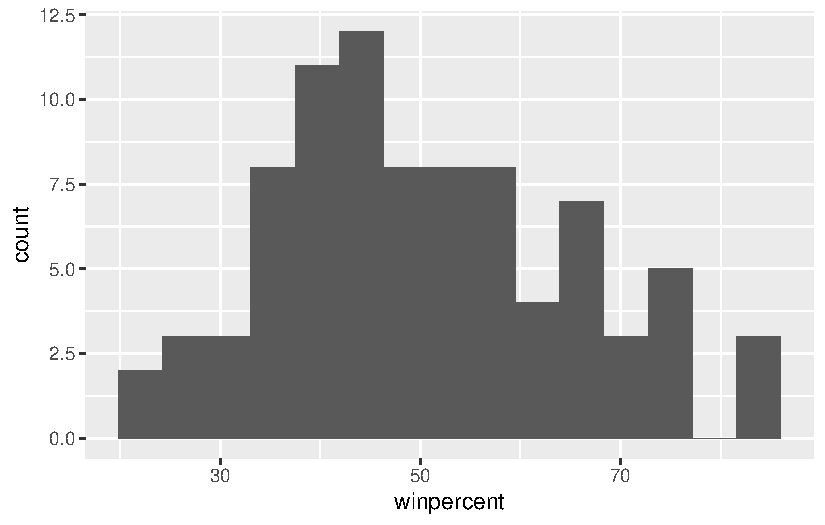
\includegraphics{halloween-mini-project_files/figure-pdf/unnamed-chunk-9-1.pdf}

}

\end{figure}

\begin{quote}
Q9: Is the distribution of win percent values symmetrical?
\end{quote}

The distribution of win percent values is skewed.

\begin{quote}
Q10: Is the center of the distribution above or below 50\%?
\end{quote}

The center of distribution is below 50\%

\begin{quote}
Q11: On average is chocolate candy higher or lower ranked than fruit
candy?
\end{quote}

First, find all chocolate candy and their \$winpercent values.

Next, summarize these values into one number.

Then, do the same for fruity candy and compare the numbers.

\begin{Shaded}
\begin{Highlighting}[]
\FunctionTok{mean}\NormalTok{(candy}\SpecialCharTok{$}\NormalTok{winpercent[}\FunctionTok{as.logical}\NormalTok{(candy}\SpecialCharTok{$}\NormalTok{chocolate)])}
\end{Highlighting}
\end{Shaded}

\begin{verbatim}
[1] 60.92153
\end{verbatim}

\begin{Shaded}
\begin{Highlighting}[]
\FunctionTok{mean}\NormalTok{(candy}\SpecialCharTok{$}\NormalTok{winpercent[}\FunctionTok{as.logical}\NormalTok{(candy}\SpecialCharTok{$}\NormalTok{fruity)])}
\end{Highlighting}
\end{Shaded}

\begin{verbatim}
[1] 44.11974
\end{verbatim}

On average, chocolate candy is ranked higher than fruity candy (60.92\%
\textgreater{} 44.12\%).

\begin{quote}
Q12: Is this difference statistically significant?
\end{quote}

\begin{Shaded}
\begin{Highlighting}[]
\FunctionTok{t.test}\NormalTok{(candy}\SpecialCharTok{$}\NormalTok{winpercent[}\FunctionTok{as.logical}\NormalTok{(candy}\SpecialCharTok{$}\NormalTok{chocolate)],candy}\SpecialCharTok{$}\NormalTok{winpercent[}\FunctionTok{as.logical}\NormalTok{(candy}\SpecialCharTok{$}\NormalTok{fruity)])}
\end{Highlighting}
\end{Shaded}

\begin{verbatim}

    Welch Two Sample t-test

data:  candy$winpercent[as.logical(candy$chocolate)] and candy$winpercent[as.logical(candy$fruity)]
t = 6.2582, df = 68.882, p-value = 2.871e-08
alternative hypothesis: true difference in means is not equal to 0
95 percent confidence interval:
 11.44563 22.15795
sample estimates:
mean of x mean of y 
 60.92153  44.11974 
\end{verbatim}

These results are statistically significant with a p-value of 2.87e-08.

\hypertarget{overall-candy-rankings}{%
\subsection{Overall Candy Rankings}\label{overall-candy-rankings}}

\begin{quote}
Q13: What are the five least liked candy types in this set?
\end{quote}

\begin{Shaded}
\begin{Highlighting}[]
\FunctionTok{library}\NormalTok{(dplyr)}
\end{Highlighting}
\end{Shaded}

\begin{verbatim}

Attaching package: 'dplyr'
\end{verbatim}

\begin{verbatim}
The following objects are masked from 'package:stats':

    filter, lag
\end{verbatim}

\begin{verbatim}
The following objects are masked from 'package:base':

    intersect, setdiff, setequal, union
\end{verbatim}

\begin{Shaded}
\begin{Highlighting}[]
\NormalTok{candy }\SpecialCharTok{\%\textgreater{}\%}
  \FunctionTok{arrange}\NormalTok{(winpercent) }\SpecialCharTok{\%\textgreater{}\%}
  \FunctionTok{head}\NormalTok{(}\DecValTok{5}\NormalTok{)}
\end{Highlighting}
\end{Shaded}

\begin{verbatim}
                   chocolate fruity caramel peanutyalmondy nougat
Nik L Nip                  0      1       0              0      0
Boston Baked Beans         0      0       0              1      0
Chiclets                   0      1       0              0      0
Super Bubble               0      1       0              0      0
Jawbusters                 0      1       0              0      0
                   crispedricewafer hard bar pluribus sugarpercent pricepercent
Nik L Nip                         0    0   0        1        0.197        0.976
Boston Baked Beans                0    0   0        1        0.313        0.511
Chiclets                          0    0   0        1        0.046        0.325
Super Bubble                      0    0   0        0        0.162        0.116
Jawbusters                        0    1   0        1        0.093        0.511
                   winpercent
Nik L Nip            22.44534
Boston Baked Beans   23.41782
Chiclets             24.52499
Super Bubble         27.30386
Jawbusters           28.12744
\end{verbatim}

The top 5 least liked candies are Nik L Nip, Boston Baked Beans,
Chiclets, Super Bubble, and Jawbusters.

\begin{quote}
Q14: What are the top 5 all time favorite candy types out of this set?
\end{quote}

\begin{Shaded}
\begin{Highlighting}[]
\NormalTok{candy }\SpecialCharTok{\%\textgreater{}\%}
  \FunctionTok{arrange}\NormalTok{(winpercent) }\SpecialCharTok{\%\textgreater{}\%}
  \FunctionTok{tail}\NormalTok{(}\DecValTok{5}\NormalTok{)}
\end{Highlighting}
\end{Shaded}

\begin{verbatim}
                          chocolate fruity caramel peanutyalmondy nougat
Snickers                          1      0       1              1      1
Kit Kat                           1      0       0              0      0
Twix                              1      0       1              0      0
Reese's Miniatures                1      0       0              1      0
Reese's Peanut Butter cup         1      0       0              1      0
                          crispedricewafer hard bar pluribus sugarpercent
Snickers                                 0    0   1        0        0.546
Kit Kat                                  1    0   1        0        0.313
Twix                                     1    0   1        0        0.546
Reese's Miniatures                       0    0   0        0        0.034
Reese's Peanut Butter cup                0    0   0        0        0.720
                          pricepercent winpercent
Snickers                         0.651   76.67378
Kit Kat                          0.511   76.76860
Twix                             0.906   81.64291
Reese's Miniatures               0.279   81.86626
Reese's Peanut Butter cup        0.651   84.18029
\end{verbatim}

The top 5 all time favorite candy types are Reese's Peanut Butter Cup,
Reese's Miniatures, Twix, Kit Kat, and Snickers.

\begin{quote}
Q15: Make a first barplot of candy ranking based on winpercent values.
\end{quote}

\begin{Shaded}
\begin{Highlighting}[]
\FunctionTok{ggplot}\NormalTok{(candy, }\FunctionTok{aes}\NormalTok{(winpercent, }\FunctionTok{rownames}\NormalTok{(candy))) }\SpecialCharTok{+}
  \FunctionTok{geom\_col}\NormalTok{()}
\end{Highlighting}
\end{Shaded}

\begin{figure}[H]

{\centering 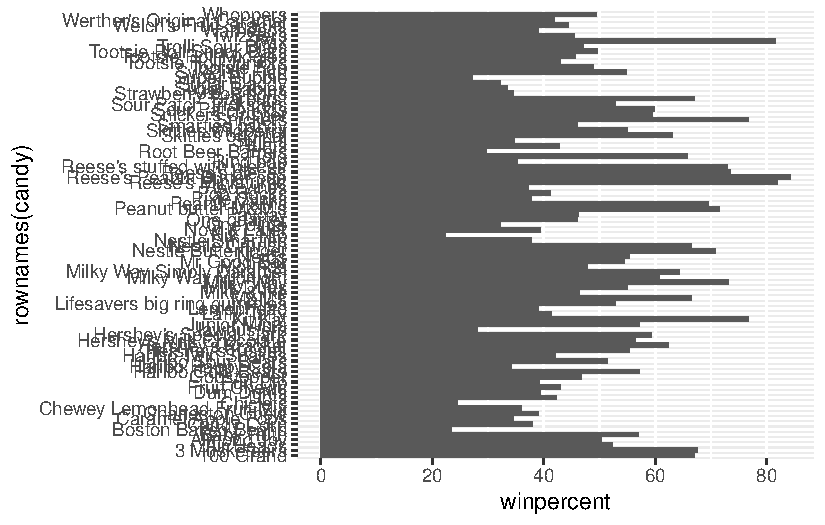
\includegraphics{halloween-mini-project_files/figure-pdf/unnamed-chunk-15-1.pdf}

}

\end{figure}

\begin{quote}
Q16: This is very ugly, use the \texttt{reorder()} function to get the
bars sorted by \texttt{winpercent}?
\end{quote}

\begin{Shaded}
\begin{Highlighting}[]
\FunctionTok{ggplot}\NormalTok{(candy, }\FunctionTok{aes}\NormalTok{(winpercent, }\FunctionTok{reorder}\NormalTok{(}\FunctionTok{rownames}\NormalTok{(candy), winpercent))) }\SpecialCharTok{+} 
  \FunctionTok{geom\_col}\NormalTok{() }\SpecialCharTok{+} 
  \FunctionTok{labs}\NormalTok{(}\AttributeTok{x =} \StringTok{"Win Percent"}\NormalTok{, }\AttributeTok{y =} \ConstantTok{NULL}\NormalTok{)}
\end{Highlighting}
\end{Shaded}

\begin{figure}[H]

{\centering 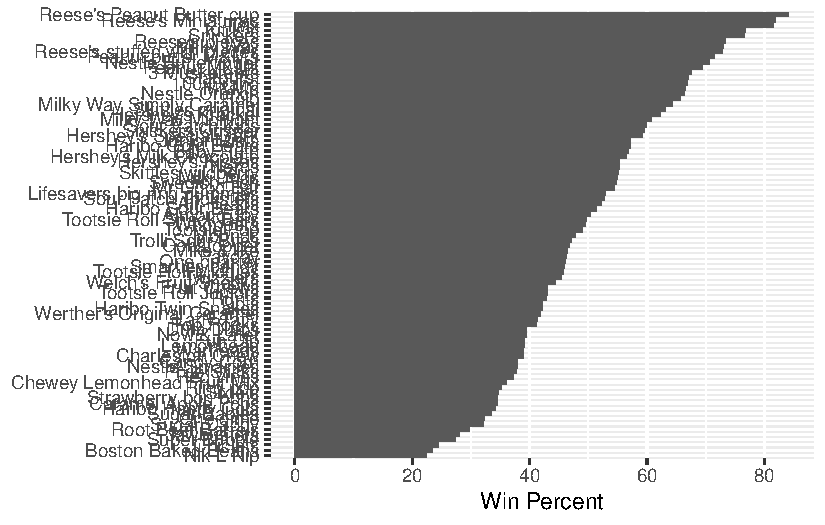
\includegraphics{halloween-mini-project_files/figure-pdf/unnamed-chunk-16-1.pdf}

}

\end{figure}

\begin{Shaded}
\begin{Highlighting}[]
\CommentTok{\# Still ugly. Can we adjust the labels so we can read them better?}
\FunctionTok{ggsave}\NormalTok{(}\StringTok{\textquotesingle{}barplot1.png\textquotesingle{}}\NormalTok{, }\AttributeTok{width =} \DecValTok{7}\NormalTok{, }\AttributeTok{height =} \DecValTok{10}\NormalTok{)}
\end{Highlighting}
\end{Shaded}

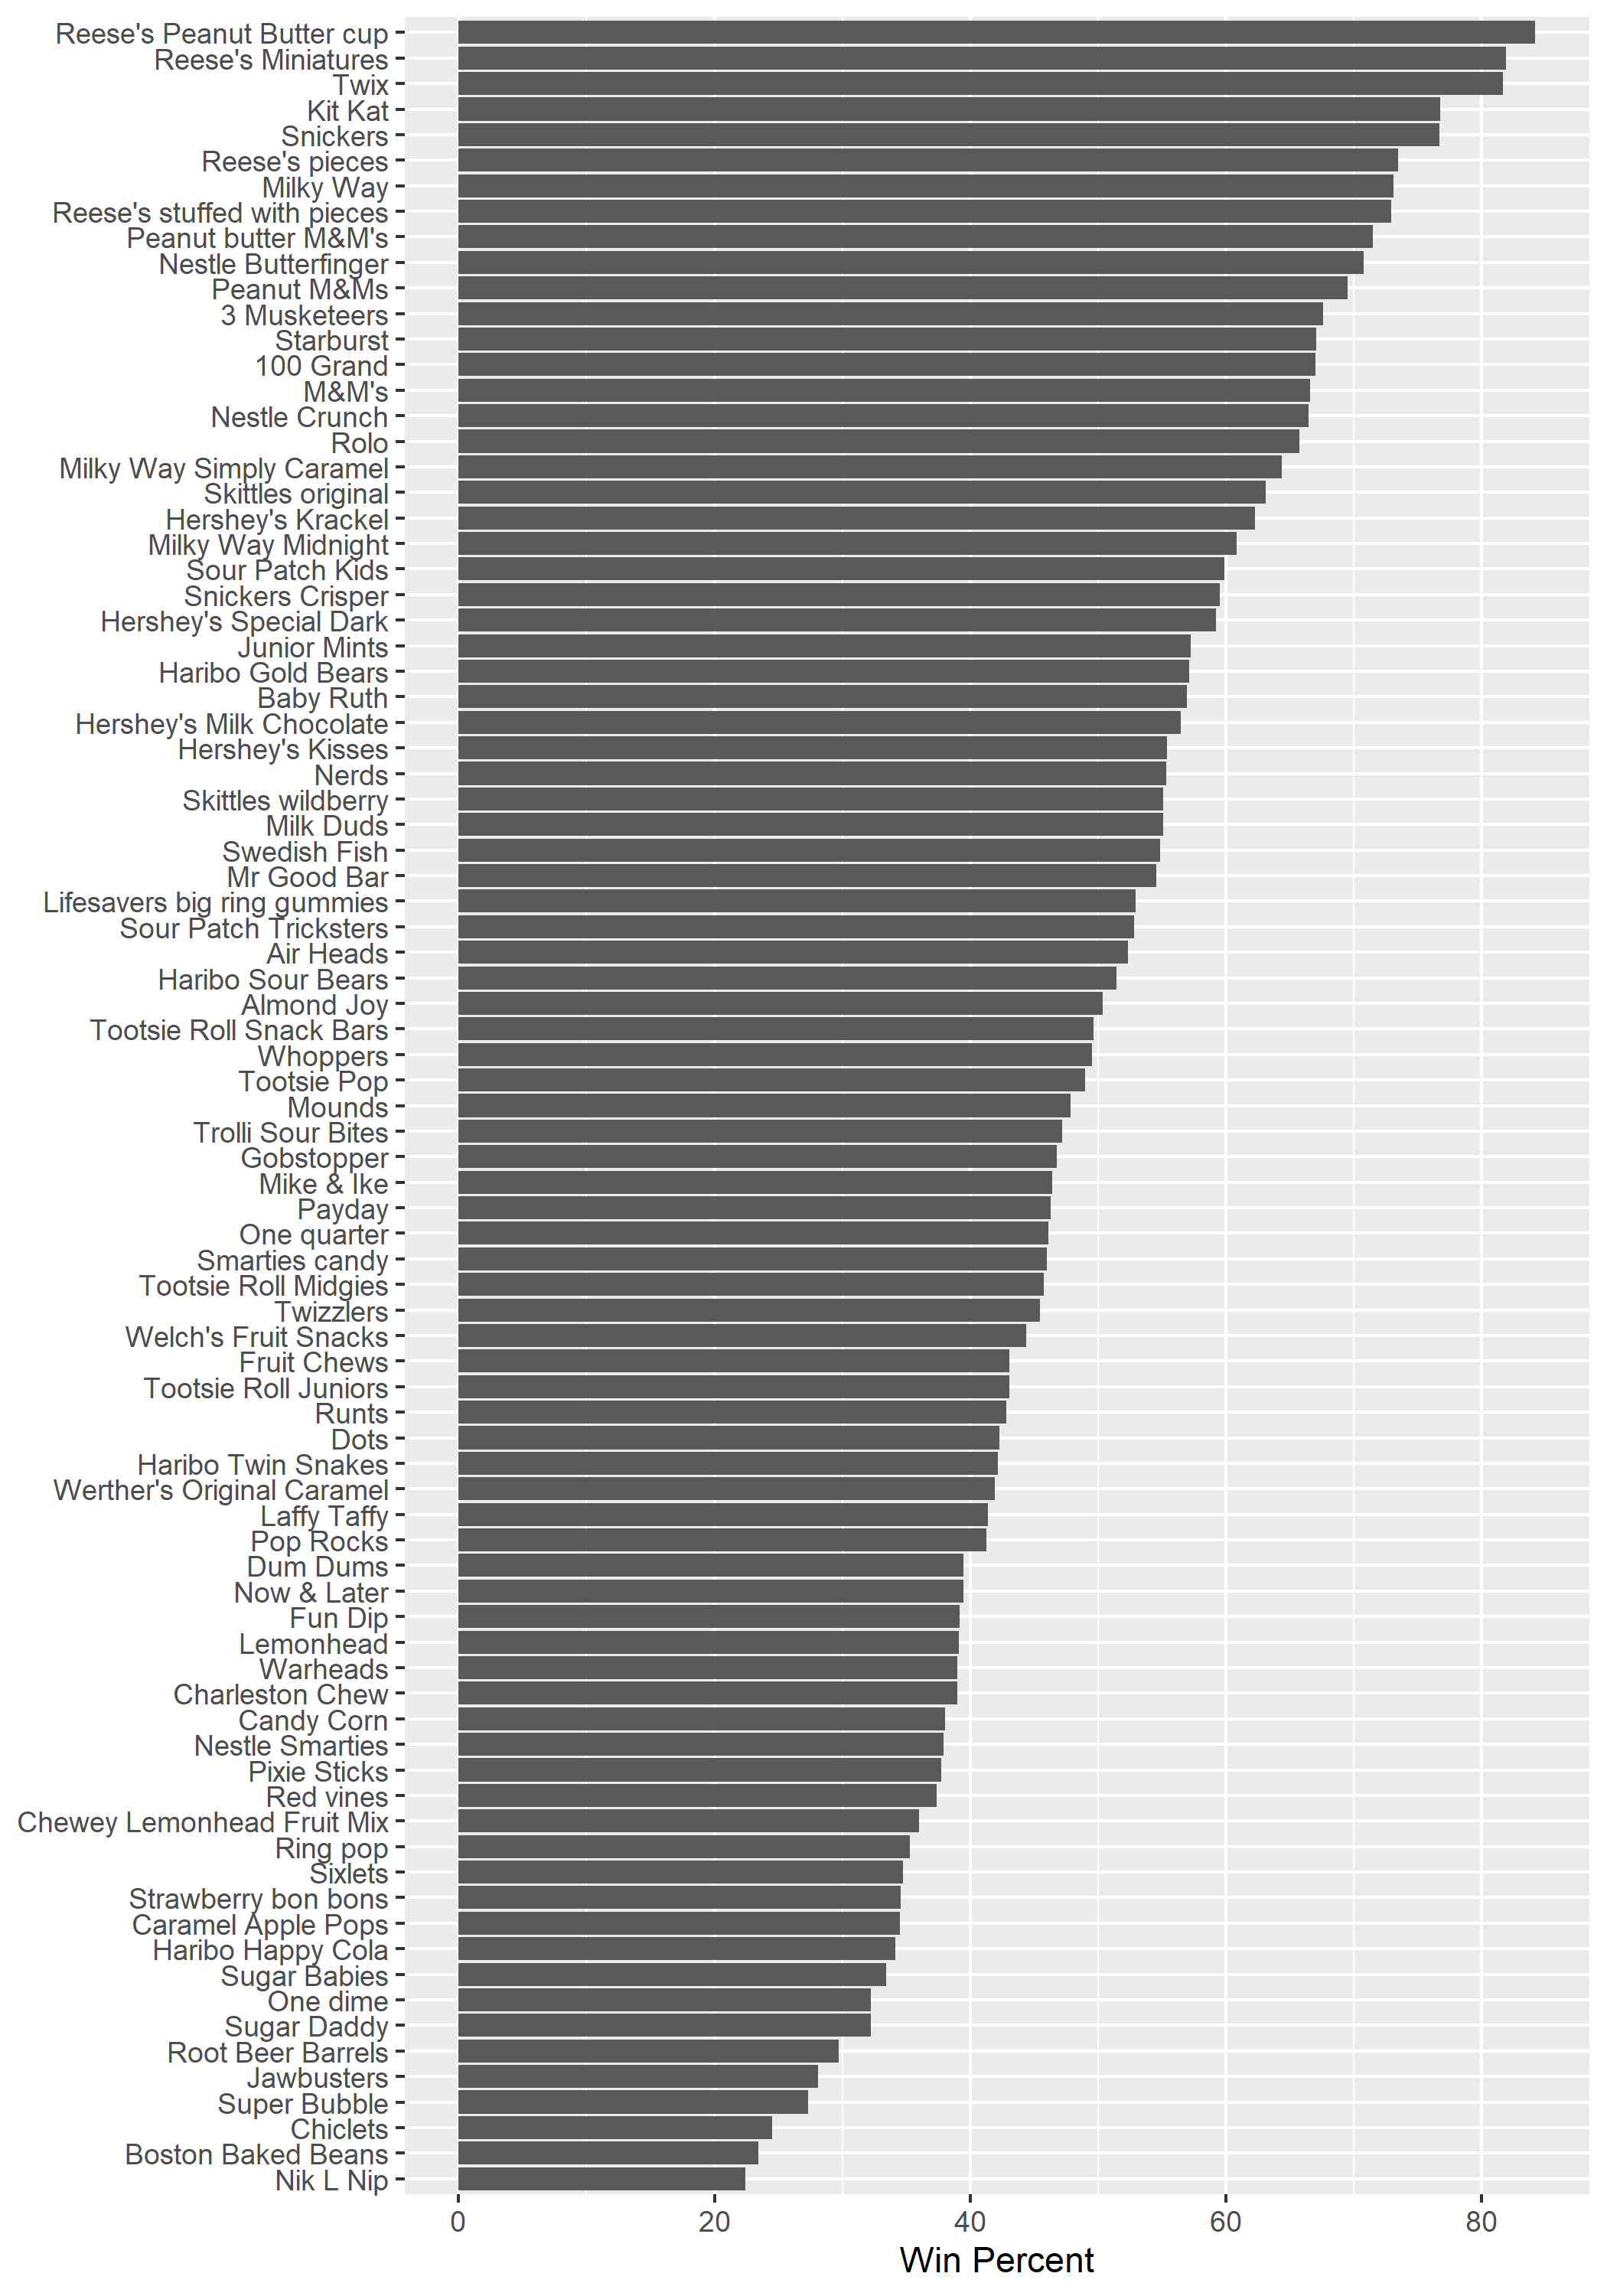
\includegraphics{barplot1.png}

You can insert any image using this markdown syntax.
\texttt{!{[}{]}(barplot1.png)}

Now let's add color to our ggplot. We need to make a custom color
vector.

\begin{Shaded}
\begin{Highlighting}[]
\CommentTok{\# Start with an all black vector of colors.}
\NormalTok{my\_cols }\OtherTok{\textless{}{-}} \FunctionTok{rep}\NormalTok{(}\StringTok{"black"}\NormalTok{, }\FunctionTok{nrow}\NormalTok{(candy))}
\NormalTok{my\_cols[}\FunctionTok{as.logical}\NormalTok{(candy}\SpecialCharTok{$}\NormalTok{chocolate)] }\OtherTok{=} \StringTok{"deeppink4"}
\NormalTok{my\_cols[}\FunctionTok{as.logical}\NormalTok{(candy}\SpecialCharTok{$}\NormalTok{bar)] }\OtherTok{=} \StringTok{"palevioletred3"}
\NormalTok{my\_cols[}\FunctionTok{as.logical}\NormalTok{(candy}\SpecialCharTok{$}\NormalTok{fruity)] }\OtherTok{=} \StringTok{"plum3"}
\end{Highlighting}
\end{Shaded}

\begin{Shaded}
\begin{Highlighting}[]
\FunctionTok{ggplot}\NormalTok{(candy, }\FunctionTok{aes}\NormalTok{(winpercent, }\FunctionTok{reorder}\NormalTok{(}\FunctionTok{rownames}\NormalTok{(candy), winpercent))) }\SpecialCharTok{+} 
  \FunctionTok{geom\_col}\NormalTok{(}\AttributeTok{fill =}\NormalTok{ my\_cols) }\SpecialCharTok{+} 
  \FunctionTok{labs}\NormalTok{(}\AttributeTok{x =} \StringTok{"Win Percent"}\NormalTok{, }\AttributeTok{y =} \ConstantTok{NULL}\NormalTok{)}
\end{Highlighting}
\end{Shaded}

\begin{figure}[H]

{\centering 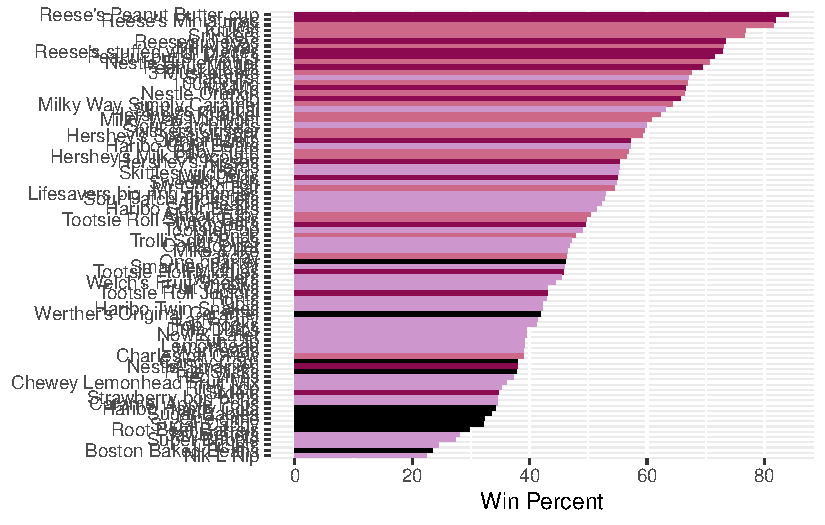
\includegraphics{halloween-mini-project_files/figure-pdf/unnamed-chunk-18-1.pdf}

}

\end{figure}

\begin{Shaded}
\begin{Highlighting}[]
\FunctionTok{ggsave}\NormalTok{(}\StringTok{\textquotesingle{}barplot2.png\textquotesingle{}}\NormalTok{, }\AttributeTok{width =} \DecValTok{7}\NormalTok{, }\AttributeTok{height =} \DecValTok{10}\NormalTok{)}
\end{Highlighting}
\end{Shaded}

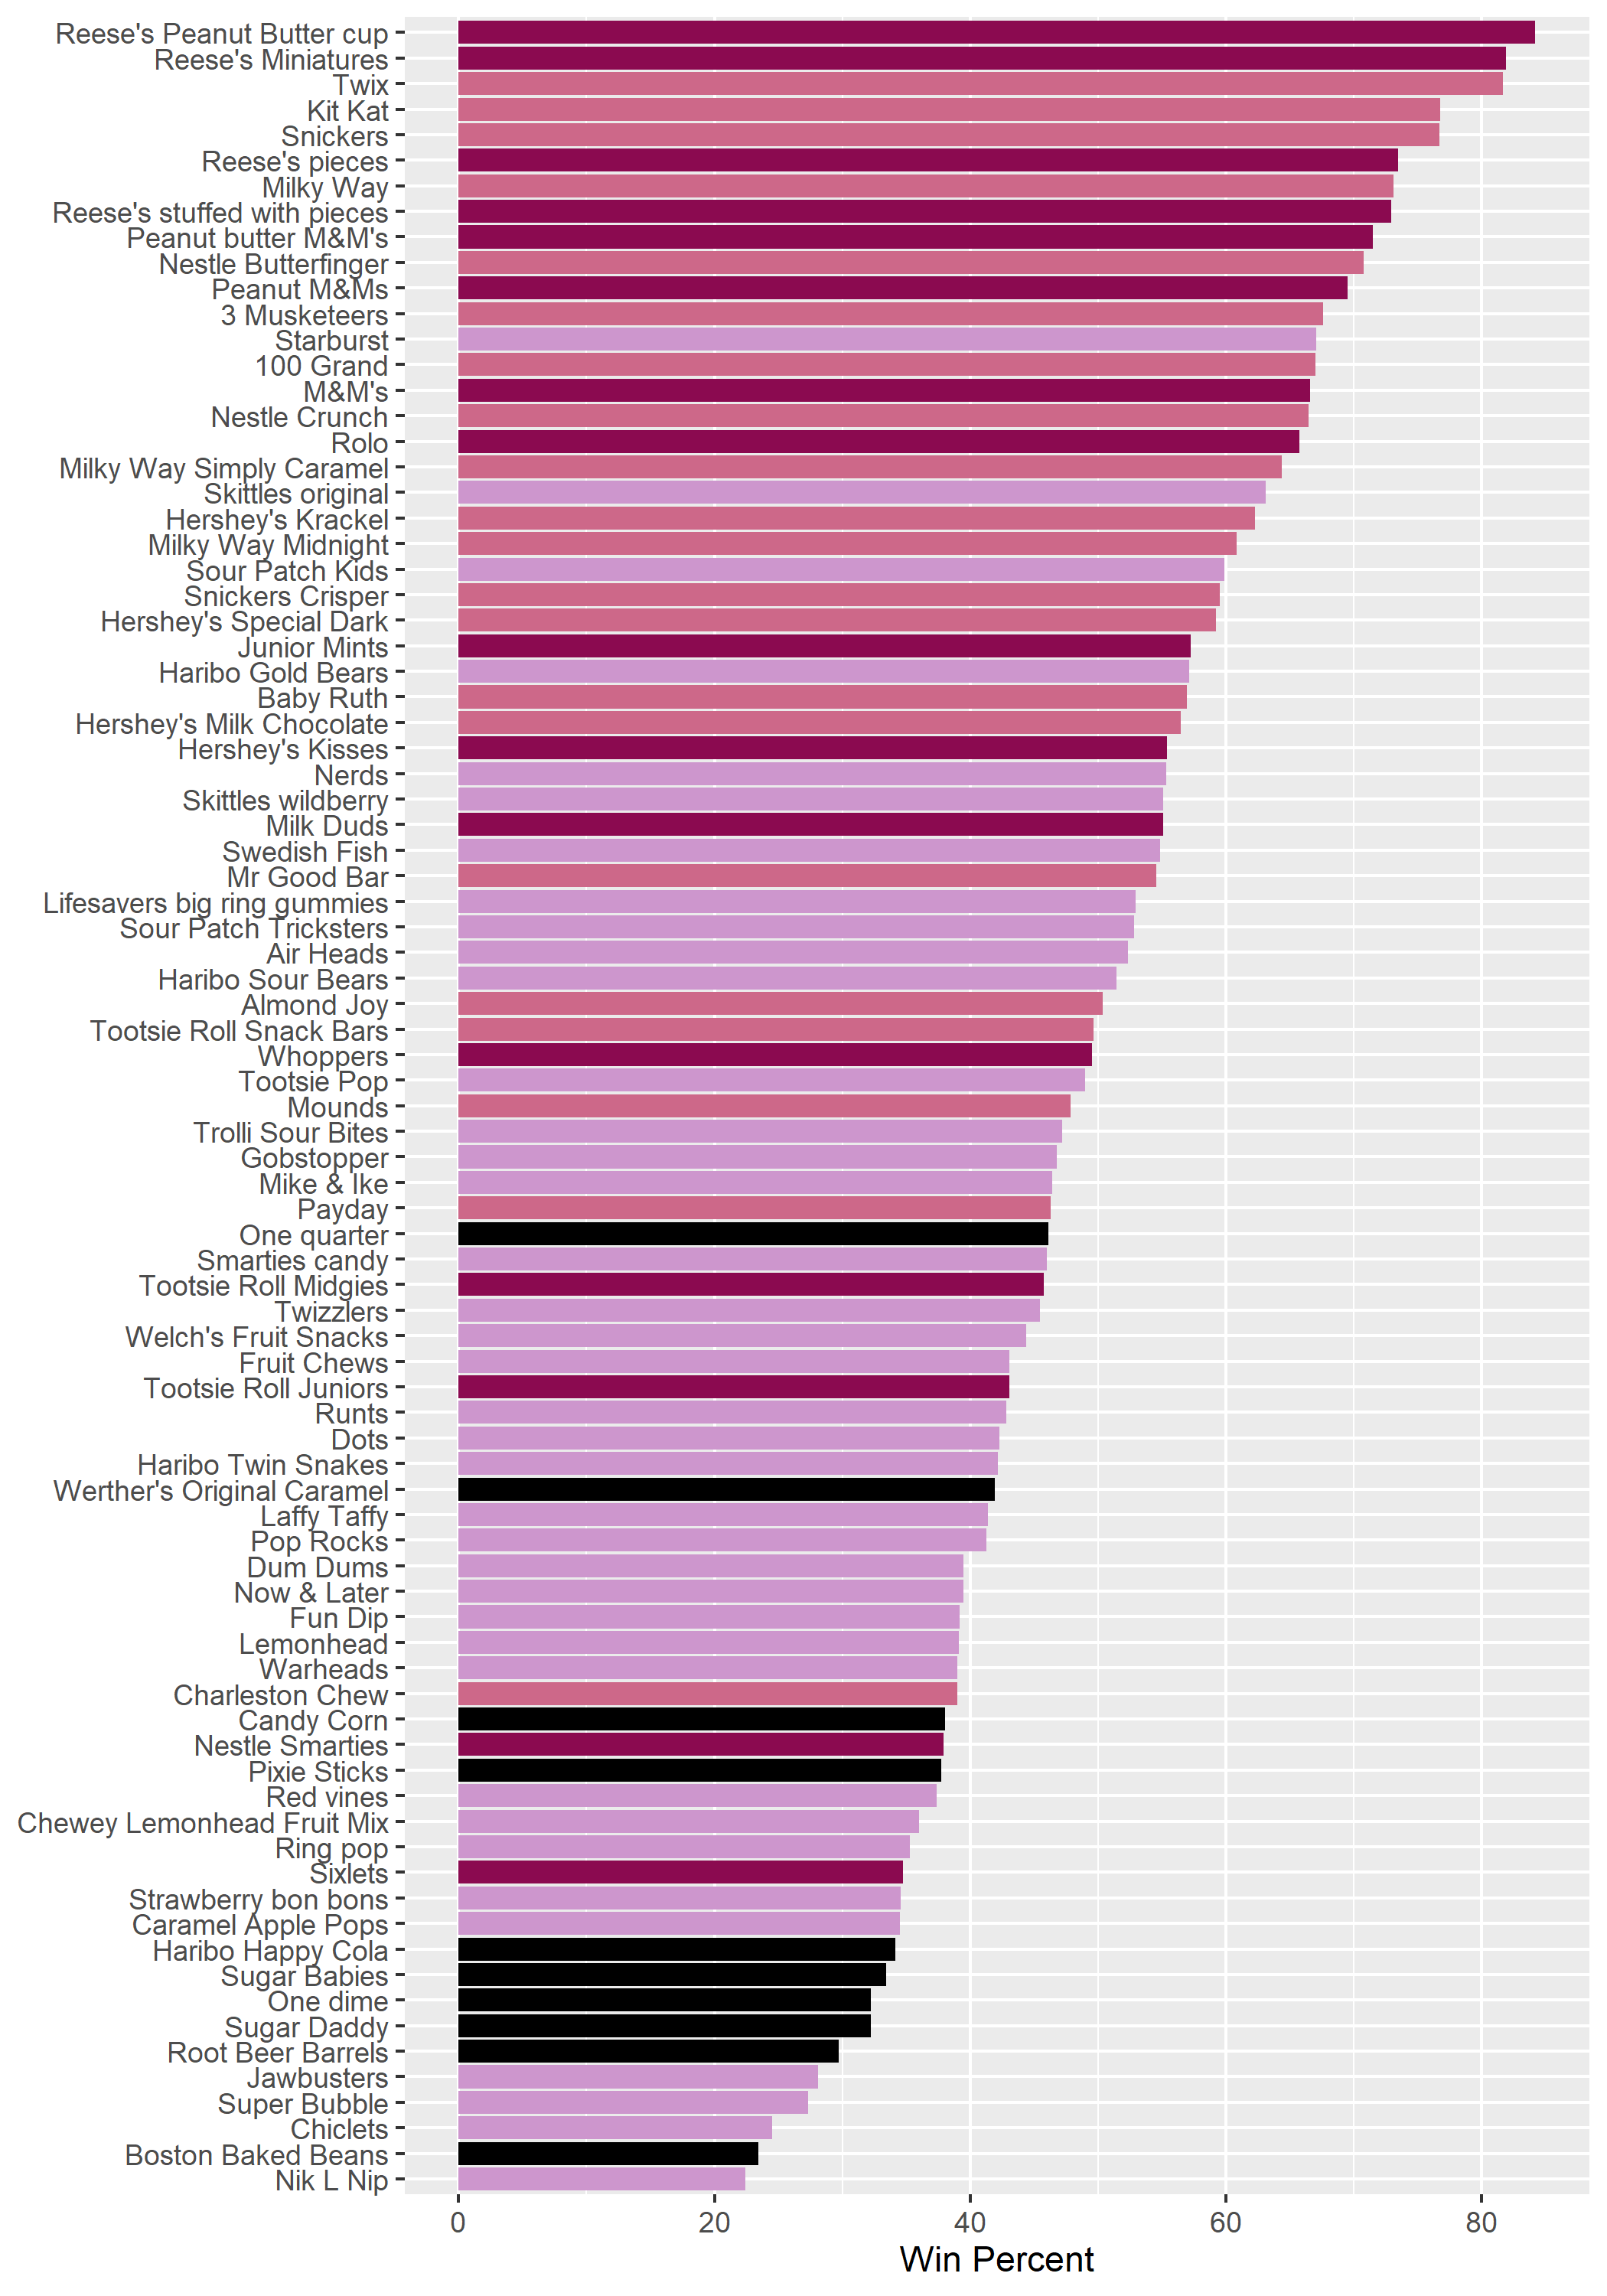
\includegraphics{barplot2.png}

\begin{quote}
Q17: What is the worst ranked chocolate candy?
\end{quote}

The worst ranked chocolate candy is Sixlets.

\begin{quote}
Q18: What is the best ranked fruity candy?
\end{quote}

The best ranked fruity candy is Starburst.

\hypertarget{taking-a-look-at-pricepercent}{%
\subsection{Taking a look at
pricepercent}\label{taking-a-look-at-pricepercent}}

\begin{Shaded}
\begin{Highlighting}[]
\NormalTok{candy}\SpecialCharTok{$}\NormalTok{pricepercent}
\end{Highlighting}
\end{Shaded}

\begin{verbatim}
 [1] 0.860 0.511 0.116 0.511 0.511 0.767 0.767 0.511 0.325 0.325 0.511 0.511
[13] 0.325 0.511 0.034 0.034 0.325 0.453 0.465 0.465 0.465 0.465 0.093 0.918
[25] 0.918 0.918 0.511 0.511 0.511 0.116 0.104 0.279 0.651 0.651 0.325 0.511
[37] 0.651 0.441 0.860 0.860 0.918 0.325 0.767 0.767 0.976 0.325 0.767 0.651
[49] 0.023 0.837 0.116 0.279 0.651 0.651 0.651 0.965 0.860 0.069 0.279 0.081
[61] 0.220 0.220 0.976 0.116 0.651 0.651 0.116 0.116 0.220 0.058 0.767 0.325
[73] 0.116 0.755 0.325 0.511 0.011 0.325 0.255 0.906 0.116 0.116 0.313 0.267
[85] 0.848
\end{verbatim}

if we want to see what is a good candy to buy in terms of winpercent and
pricepercent, we can plot these two variables and then see the best
candy for the least amount of money.

\begin{Shaded}
\begin{Highlighting}[]
\FunctionTok{ggplot}\NormalTok{(candy) }\SpecialCharTok{+} 
  \FunctionTok{aes}\NormalTok{(winpercent, pricepercent, }\AttributeTok{label=}\FunctionTok{rownames}\NormalTok{(candy)) }\SpecialCharTok{+}
  \FunctionTok{geom\_point}\NormalTok{(}\AttributeTok{col=}\NormalTok{my\_cols) }\SpecialCharTok{+}
  \FunctionTok{geom\_text}\NormalTok{()}
\end{Highlighting}
\end{Shaded}

\begin{figure}[H]

{\centering 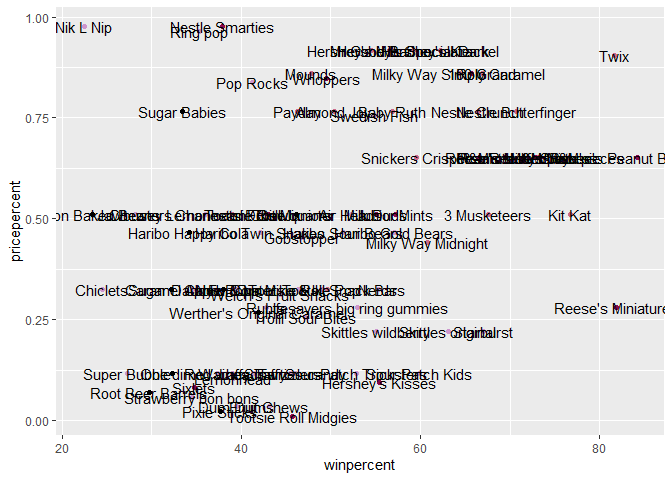
\includegraphics{halloween-mini-project_files/figure-pdf/unnamed-chunk-21-1.pdf}

}

\end{figure}

To avoid the overplotting of all these labels we can use an add on
package called ggrepl.

\begin{Shaded}
\begin{Highlighting}[]
\FunctionTok{library}\NormalTok{(ggrepel)}
\FunctionTok{ggplot}\NormalTok{(candy) }\SpecialCharTok{+} 
  \FunctionTok{aes}\NormalTok{(winpercent, pricepercent, }\AttributeTok{label=}\FunctionTok{rownames}\NormalTok{(candy)) }\SpecialCharTok{+}
  \FunctionTok{geom\_point}\NormalTok{(}\AttributeTok{col=}\NormalTok{my\_cols) }\SpecialCharTok{+}
  \FunctionTok{geom\_text\_repel}\NormalTok{()}
\end{Highlighting}
\end{Shaded}

\begin{verbatim}
Warning: ggrepel: 50 unlabeled data points (too many overlaps). Consider
increasing max.overlaps
\end{verbatim}

\begin{figure}[H]

{\centering 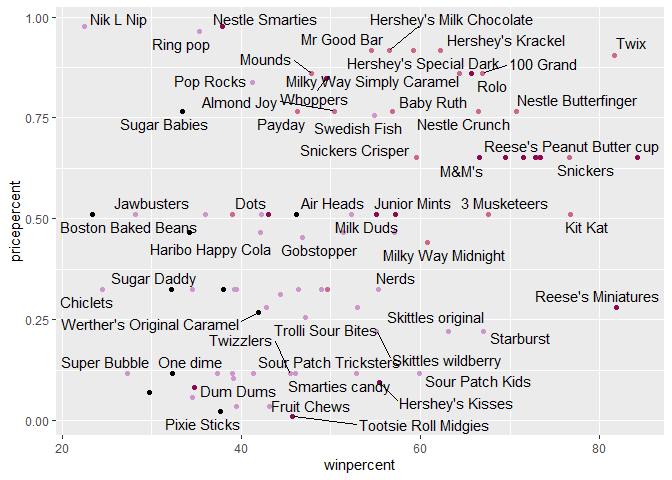
\includegraphics{halloween-mini-project_files/figure-pdf/unnamed-chunk-22-1.pdf}

}

\end{figure}

Play with the \texttt{max.overlaps} parameter on
\texttt{geom\_text\_repel}.

\begin{Shaded}
\begin{Highlighting}[]
\FunctionTok{ggplot}\NormalTok{(candy) }\SpecialCharTok{+} 
  \FunctionTok{aes}\NormalTok{(winpercent, pricepercent, }\AttributeTok{label=}\FunctionTok{rownames}\NormalTok{(candy)) }\SpecialCharTok{+}
  \FunctionTok{geom\_point}\NormalTok{(}\AttributeTok{col=}\NormalTok{my\_cols) }\SpecialCharTok{+}
  \FunctionTok{geom\_text\_repel}\NormalTok{(}\AttributeTok{max.overlaps=}\DecValTok{5}\NormalTok{, }\AttributeTok{col=}\NormalTok{my\_cols, }\AttributeTok{size =} \FloatTok{3.3}\NormalTok{)}
\end{Highlighting}
\end{Shaded}

\begin{verbatim}
Warning: ggrepel: 65 unlabeled data points (too many overlaps). Consider
increasing max.overlaps
\end{verbatim}

\begin{figure}[H]

{\centering 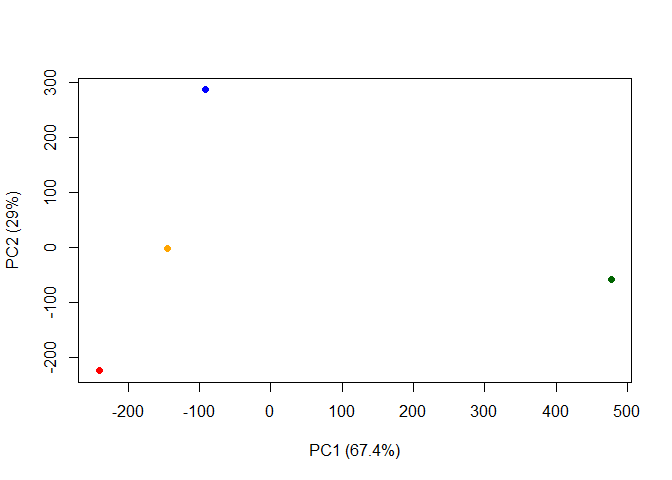
\includegraphics{halloween-mini-project_files/figure-pdf/unnamed-chunk-23-1.pdf}

}

\end{figure}

\begin{quote}
Q19: Which candy type is the highest ranked in terms of winpercent for
the least money - i.e.~offers the most bang for your buck?
\end{quote}

Reese's miniatures have the highest \texttt{winpercent} for the lowest
\texttt{pricepercent}.

\begin{quote}
Q20: What are the top 5 most expensive candy types in the dataset and of
these which is the least popular?
\end{quote}

\begin{Shaded}
\begin{Highlighting}[]
\NormalTok{ord }\OtherTok{\textless{}{-}} \FunctionTok{order}\NormalTok{(candy}\SpecialCharTok{$}\NormalTok{pricepercent, }\AttributeTok{decreasing =} \ConstantTok{TRUE}\NormalTok{)}
\FunctionTok{head}\NormalTok{( candy[ord,}\FunctionTok{c}\NormalTok{(}\DecValTok{11}\NormalTok{,}\DecValTok{12}\NormalTok{)], }\AttributeTok{n=}\DecValTok{5}\NormalTok{ )}
\end{Highlighting}
\end{Shaded}

\begin{verbatim}
                         pricepercent winpercent
Nik L Nip                       0.976   22.44534
Nestle Smarties                 0.976   37.88719
Ring pop                        0.965   35.29076
Hershey's Krackel               0.918   62.28448
Hershey's Milk Chocolate        0.918   56.49050
\end{verbatim}

The top 5 most expensive candies are Nik L Nip, Nestle Smarties, Ring
pop, Hershey's Krackel, and Hershey's Milk Chocolate. The least popular
of these is Nik L Nip.

\hypertarget{exploring-the-correlation-structure.}{%
\section{5 Exploring the correlation
structure.}\label{exploring-the-correlation-structure.}}

\begin{Shaded}
\begin{Highlighting}[]
\FunctionTok{library}\NormalTok{(corrplot)}
\end{Highlighting}
\end{Shaded}

\begin{verbatim}
corrplot 0.92 loaded
\end{verbatim}

\begin{Shaded}
\begin{Highlighting}[]
\NormalTok{cij }\OtherTok{\textless{}{-}} \FunctionTok{cor}\NormalTok{(candy)}
\FunctionTok{corrplot}\NormalTok{(cij)}
\end{Highlighting}
\end{Shaded}

\begin{figure}[H]

{\centering 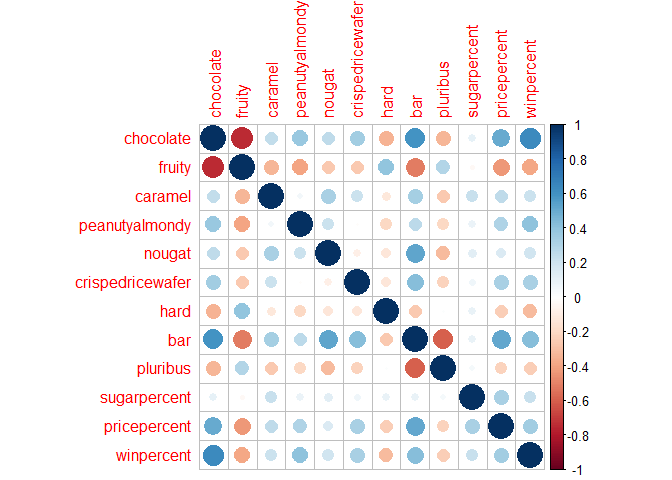
\includegraphics{halloween-mini-project_files/figure-pdf/unnamed-chunk-25-1.pdf}

}

\end{figure}

\begin{quote}
Q22: Examining this plot what two variables are anti-correlated
(i.e.~have minus values)?
\end{quote}

Fruity and chocolate are two variables that are anticorrelated.

\begin{quote}
Q23: Similarly, what two variables are most positively correlated?
\end{quote}

Chocolate and winpercent are the two variables that are the most
positively correlated.

\hypertarget{on-to-pca}{%
\section{On to PCA}\label{on-to-pca}}

The main function for this is called \texttt{prcom()} and here we know
we need to scale our data with the \texttt{scale=TRUE} argument.

\begin{Shaded}
\begin{Highlighting}[]
\NormalTok{pca }\OtherTok{\textless{}{-}} \FunctionTok{prcomp}\NormalTok{(candy, }\AttributeTok{scale=}\ConstantTok{TRUE}\NormalTok{)}
\FunctionTok{summary}\NormalTok{(pca)}
\end{Highlighting}
\end{Shaded}

\begin{verbatim}
Importance of components:
                          PC1    PC2    PC3     PC4    PC5     PC6     PC7
Standard deviation     2.0788 1.1378 1.1092 1.07533 0.9518 0.81923 0.81530
Proportion of Variance 0.3601 0.1079 0.1025 0.09636 0.0755 0.05593 0.05539
Cumulative Proportion  0.3601 0.4680 0.5705 0.66688 0.7424 0.79830 0.85369
                           PC8     PC9    PC10    PC11    PC12
Standard deviation     0.74530 0.67824 0.62349 0.43974 0.39760
Proportion of Variance 0.04629 0.03833 0.03239 0.01611 0.01317
Cumulative Proportion  0.89998 0.93832 0.97071 0.98683 1.00000
\end{verbatim}

\begin{Shaded}
\begin{Highlighting}[]
\NormalTok{my\_data }\OtherTok{\textless{}{-}} \FunctionTok{cbind}\NormalTok{(candy, pca}\SpecialCharTok{$}\NormalTok{x[,}\DecValTok{1}\SpecialCharTok{:}\DecValTok{3}\NormalTok{])}
\end{Highlighting}
\end{Shaded}

\begin{Shaded}
\begin{Highlighting}[]
\FunctionTok{ggplot}\NormalTok{(my\_data) }\SpecialCharTok{+}
  \FunctionTok{aes}\NormalTok{(PC1, PC2, }\AttributeTok{label =} \FunctionTok{rownames}\NormalTok{(candy)) }\SpecialCharTok{+}
  \FunctionTok{geom\_point}\NormalTok{(}\AttributeTok{col=}\NormalTok{my\_cols) }\SpecialCharTok{+}
  \FunctionTok{geom\_text\_repel}\NormalTok{(}\AttributeTok{col=}\NormalTok{my\_cols) }\SpecialCharTok{+}
  \FunctionTok{labs}\NormalTok{(}\AttributeTok{title=}\StringTok{"PCA Candy Space Map"}\NormalTok{, }\AttributeTok{subtitle =} \StringTok{"Colored by type: chocolate bar (pink), chocolate other (burgundy), fruity (lavender), other (black)"}\NormalTok{, }\AttributeTok{caption=} \StringTok{"Data from 538"}\NormalTok{)}
\end{Highlighting}
\end{Shaded}

\begin{verbatim}
Warning: ggrepel: 56 unlabeled data points (too many overlaps). Consider
increasing max.overlaps
\end{verbatim}

\begin{figure}[H]

{\centering 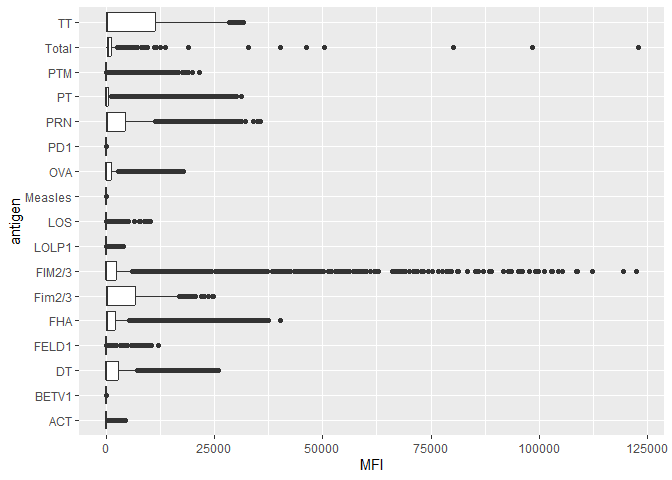
\includegraphics{halloween-mini-project_files/figure-pdf/unnamed-chunk-28-1.pdf}

}

\end{figure}

\hypertarget{loadings-plot}{%
\subsection{Loadings Plot}\label{loadings-plot}}

\begin{Shaded}
\begin{Highlighting}[]
\NormalTok{loadings }\OtherTok{\textless{}{-}} \FunctionTok{as.data.frame}\NormalTok{(pca}\SpecialCharTok{$}\NormalTok{rotation)}

\FunctionTok{ggplot}\NormalTok{(loadings) }\SpecialCharTok{+}
  \FunctionTok{aes}\NormalTok{(PC1, }\FunctionTok{reorder}\NormalTok{(}\FunctionTok{rownames}\NormalTok{(loadings), PC1)) }\SpecialCharTok{+}
  \FunctionTok{geom\_col}\NormalTok{()}
\end{Highlighting}
\end{Shaded}

\begin{figure}[H]

{\centering 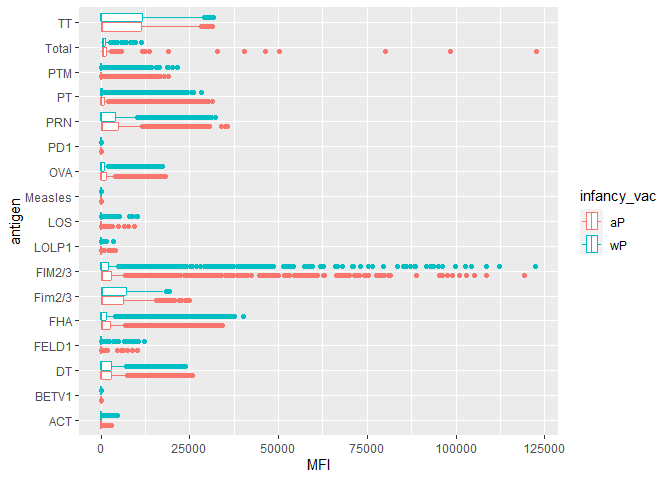
\includegraphics{halloween-mini-project_files/figure-pdf/unnamed-chunk-29-1.pdf}

}

\end{figure}

\begin{quote}
Q24: What original variables are picked up strongly by PC1 in the
positive direction? Do these make sense to you?
\end{quote}

The fruity, pluribus, and hard variables are picked up strongly by PC1
in the positive direction. This makes sense, as these variables are all
correlated with each other, whereas the remaining variables in the
negative direction are all correlated with each other.



\end{document}
